\section{Dilemmas and Trilemmas\label{sec:dilemma_trilemma}}

A simple decision is one that has one good choice and one or more bad choices. The work is to identify which is the good choice and select that option.

A complex decision may have many choices, and there are might not be a best option. Then a Pareto frontier might exist where trade-offs can be made. 

When a decision has two viable options (neither being best), that presents a \href{https://en.wikipedia.org/wiki/Dilemma}{dilemma}. The name for the case with three viable options is a \href{https://en.wikipedia.org/wiki/Trilemma}{trilemma}.

Dilemmas create cognitive dissonance for the decision maker. Any selection is going to have downsides, and any compromise will be suboptimal. 

The following are presented as dilemmas, but that oversimplifies both the continuous nature of the trade-off and the alternative creative approaches to a specific situation. The reason to be aware of these dilemmas to be able to ponder them prior to the pressure of real-time decision making. 

The dilemmas are all happening at the same time and all the time, and they are inter-dependent. Making a choice for one dilemma shapes the options available in other dilemmas.

These dilemmas are presented in no particular order. 

\ \\

\begin{center}
\begin{table}[ht]
\begin{tabular}{ | m{\dilemmatablewidth}| m{\dilemmatablewidth} | } 
  \hline
  \textbf{Control via rules} & \textbf{freedom/autonomy/agility} \\ 
  \hline
  \textit{description}: high number of rules to cover a variety of situations & 
  \textit{description}: low number of rules to enable flexibility \\ 
  \hline
  \textit{Cons}: The more rules that exist the more likely it is that someone will find a way to exploit them to their own advantage. & 
  \textit{Cons}: The fewer rules that exist the more likely it is that someone will try to get away with something bad. \\  
  \hline
\end{tabular}
\caption{Number of rules.
{\tiny Organization's culture}
}
\end{table}
\end{center}
Alternative approach: guidance derived from principles that can be adapted to specific situations. That has the problem of requiring good knowledge of the situation and wise judgement.


\ \\

\begin{center}
\begin{table}[ht]
\begin{tabular}{ | m{\dilemmatablewidth}| m{\dilemmatablewidth} | } 
  \hline
  \textbf{rules enforced strictly} & 
  \textbf{lax rule enforcement} \\ 
  \hline
  \textit{Pros}: Predictable &
  \textit{Pros}: Bureaucrats feel empowered. \\
  \hline
  \textit{Cons}: Insensitive to nuance. & 
  \textit{Cons}: Tolerance for changing conditions.  \\  
  \hline
\end{tabular}
\caption{Strictness of rules.
{\tiny Organization's culture; Processes}
}
\end{table}
\end{center}

\ \\

\begin{center}
\begin{table}[ht]
\begin{tabular}{ | m{\dilemmatablewidth}| m{\dilemmatablewidth} | } 
  \hline
  \textbf{Guidance updated frequently} & 
  \textbf{Rules persist} \\ 
  \hline
  \textit{Pros}: Adapt to new information. &
  \textit{Pros}: Stability is easier to predict. Takes less work. \\
  \hline
  \textit{Cons}: More work needed. & 
  \textit{Cons}: Doesn't adapt as conditions change. \\  
  \hline
\end{tabular}
\caption{Refresh rate of rules. See \S~\ref{sec:static-dynamic_processes}.
{\tiny Organization's culture; Processes}
}
\end{table}
\end{center}

\ \\

\begin{center}
\begin{table}[ht]
\begin{tabular}{ | m{\dilemmatablewidth}| m{\dilemmatablewidth} | } 
  \hline
  \textbf{Flatter hierarchical organization} & \textbf{More layers of hierarchy} \\ 
  \hline
  \textit{description}: more people managed per supervisor & 
  \textit{description}: fewer people managed per supervisor \\ 
  \hline
  \textit{Cons}: Less feedback/attention per employee. & 
  \textit{Cons}: Fewer people doing work. \\  
  \hline
\end{tabular}
\caption{Shape of hierarchical organization.
{\tiny Organization's culture}
}
\end{table}
\end{center}

\ \\

\begin{center}
\begin{table}[ht]
\begin{tabular}{ | m{\dilemmatablewidth}| m{\dilemmatablewidth} | } 
  \hline
  \textbf{Quickly complete tasks} & \textbf{Methodically complete tasks} \\ 
  \hline
  \textit{description}: implementing a solution quickly to address urgent needs &
  \textit{description}: Methodical well-planned design and execution \\
  \hline
  \textit{Pros}: rapid solution &
  \textit{Pros}: more like to get the solution right \\
  \hline
  \textit{Cons}: Risk of quick task is that the result is ineffective, inefficient, or wrong &
  \textit{Cons}: \href{https://en.wikipedia.org/wiki/Opportunity_cost}{opportunity cost} \\  
  \hline
\end{tabular}
\caption{Speed of task completion.
{\tiny Personal choice.}
}
\end{table}
\end{center}

\ \\

\begin{center}
\begin{table}[ht]
\begin{tabular}{ | m{\dilemmatablewidth}| m{\dilemmatablewidth} | } 
  \hline
  \textbf{Gather lots of data} &
  \textbf{Gather minimal data} \\
  \hline
  \textit{description}: Gather lots of data for a well-informed decision &
  \textit{description}: Minimal information because decision maker knows what to do or outcome is irrelevant.  \\  
  \hline
  \textit{Cons}: High cost of gathering data (time, resources). Opportunity costs. & 
  \textit{Cons}: Lack of data results in decisions based on oversimplified assessment \\
  \hline
\end{tabular}
\caption{How much data to gather for a decision. See \S~\ref{sec:bureaucratic_debt}.
{\tiny Tag: decision making; Processes}
}
\label{table:gather_data_lots-vs-little}
\end{table}
\end{center}

\begin{center}
    \begin{figure}
        \centering
        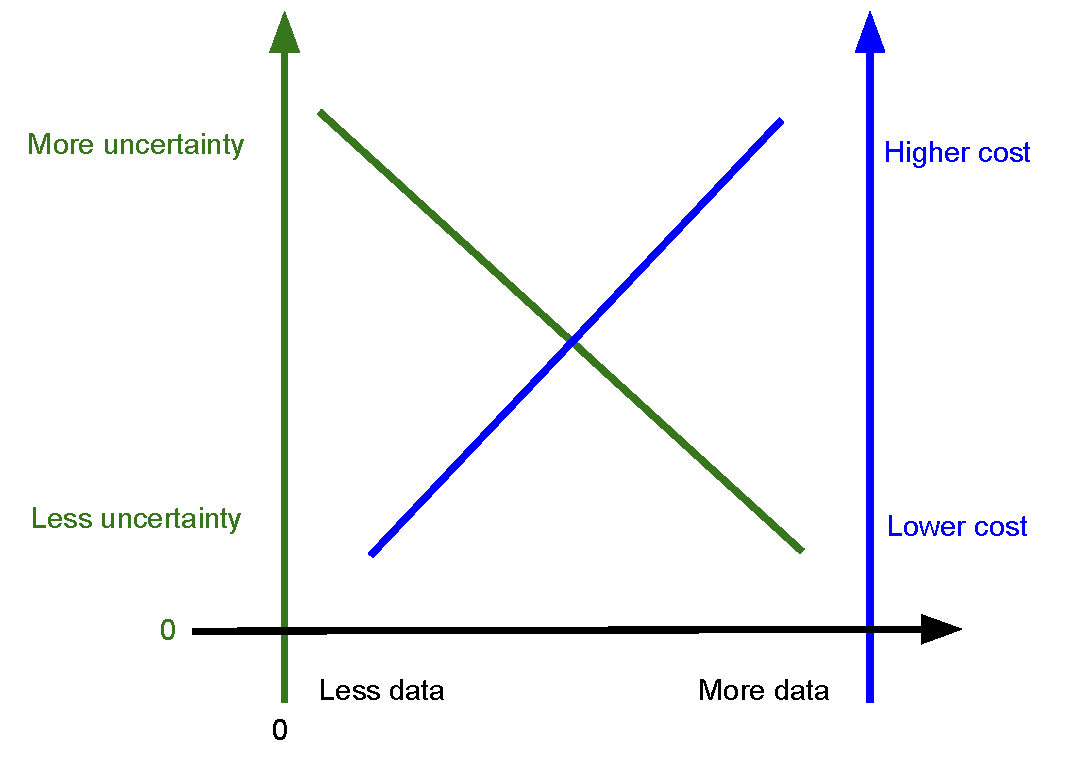
\includegraphics[width=0.8\textwidth]{images/cost_and_uncertainty_for_data_collection}
        \caption{Collecting more data costs money and decrease uncertainty.}
        \label{fig:my_label}
    \end{figure}
\end{center}

 \ \\

\begin{center}
\begin{table}[ht]
\begin{tabular}{ | m{\dilemmatablewidth}| m{\dilemmatablewidth} | } 
  \hline
  \textbf{Share less data} &
  \textbf{Share more data} \\
  \hline
  \textit{description}:  &
  \textit{description}:  \\  
  \hline
  \textit{Pros}: Restricting data access saves money for the data owner and improves flexibility.&
  \textit{Pros}: Sharing data improves transparency and accountability. \\
  \hline
  \textit{Cons}: Other people (inside and outside the organization) are unable to extract maximum value from data & 
  \textit{Cons}: Sharing data cost resources (people, money, time) \\
  \hline
\end{tabular}
\caption{How much data to share.
{\tiny Tag: Personal choice.  Processes}
}
\label{table:data_share-vs-hide}
\end{table}
\end{center}

\ \\


\begin{center}
\begin{table}[ht]
\begin{tabular}{ | m{\dilemmatablewidth}| m{\dilemmatablewidth} | } 
  \hline
  \textbf{broad scope of impact} &
  \textbf{narrow scope of impact} \\
  \hline
  \textit{description}:  &
  \textit{description}:  \\  
  \hline
  \textit{Pros}:  &
  \textit{Pros}: Niche impact means less dependencies on other people. \\
  \hline
  \textit{Cons}: & 
  \textit{Cons}: \\
  \hline
\end{tabular}
\caption{Scope of impact of your work. 
{\tiny Tag: personal choice}}
\end{table}
\label{table:scope_broad-vs-narrow}
\end{center}

\ \\

\begin{center}
\begin{table}[ht]
\begin{tabular}{ | m{\dilemmatablewidth}| m{\dilemmatablewidth} | } 
  \hline
  \textbf{staffing: good coverage} &
  \textbf{staffing: minimal coverage} \\
  \hline
  \textit{description}: sufficient staff &
  \textit{description}: as small of staff as possible \\  
  \hline
  \textit{Pros}: cover all edge cases; resilient to changing demands &
  \textit{Pros}: less expensive \\
  \hline
  \textit{Cons}: slack resources; sometimes inefficient. Increased communication needed & 
  \textit{Cons}: fragile when requirements change or workload increases. If one person departs and there's no redundancy, capacity and capability are harmed.  \\
  \hline
\end{tabular}
\caption{Size of team or organization.
{\tiny design of organization.}
}
\label{table:staff_many-vs-few}
\end{table}
\end{center}


\ \\

\begin{center}
\begin{table}[ht]
\begin{tabular}{ | m{\dilemmatablewidth}| m{\dilemmatablewidth} | } 
  \hline
  \textbf{in-house services for non-central activities } &
  \textbf{external dependencies for non-central activities} \\
  \hline
  \textit{description}:  &
  \textit{description}:  \\  
  \hline
  \textit{Pros}: More control &
  \textit{Pros}: Easier to replace \\
  \hline
  \textit{Cons}: Expands scope of responsibilities & 
  \textit{Cons}: Less understanding of problem.  \\
  \hline
\end{tabular}
\caption{Services that are necessary but not central.
{\tiny design of organization.}
}
\label{table:inhouse-vs-external}
\end{table}
\end{center}

\ \\

\begin{center}
\begin{table}[ht]
\begin{tabular}{ | m{\dilemmatablewidth}| m{\dilemmatablewidth} | } 
  \hline
  \textbf{Centralized services} &
  \textbf{Locally distributed services} \\
  \hline
  \textit{description}: A single provider of services for the organization &
  \textit{description}: Each team has a local service provider \\  
  \hline
  \textit{Pros}: Cheaper &
  \textit{Pros}: Quicker response. Accounts for local deviations from the norm \\
  \hline
  \textit{Cons}: less sensitive to local issues; less responsive & 
  \textit{Cons}: Uneven quality of service \\
  \hline
\end{tabular}
\caption{Centralization of services. See Fig.~\ref{fig:central-vs-distributed}.
{\tiny design of organization.}
}
\label{table:central-vs-distributed}
\end{table}
\end{center}

\begin{figure}[ht]
    \centering
    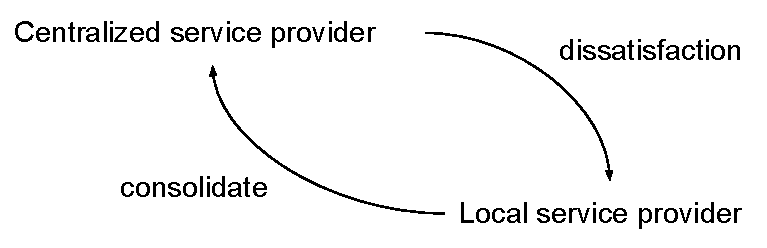
\includegraphics[width=0.8\textwidth]{images/dilemma_centralization-vs-distributed.pdf}
    \caption{Dipole oscillation. See Table~\ref{table:central-vs-distributed}}
    \label{fig:central-vs-distributed}
\end{figure}

\ \\

\begin{center}
\begin{table}[ht]
\begin{tabular}{ | m{\dilemmatablewidth}| m{\dilemmatablewidth} | } 
  \hline
  \textbf{Decision making lower in a hierarchy} &
  \textbf{Decision making higher in a hierarchy} \\
  \hline
  \textit{description}: Push decisions down to empower employees. &
  \textit{description}: Escalate every decision to management. \\  
  \hline
  \textit{Pros}: better information &
  \textit{Pros}: better scope \\
  \hline
  \textit{Cons}: more inconsistency & 
  \textit{Cons}: Decision maker has less skin in the game and may be less well informed. Employees are disempowered. \\
  \hline
\end{tabular}
\caption{Where decisions get made in hierarchical organization.
{\tiny design of organization.}
}
\label{table:decisions_low-vs-high}
\end{table}
\end{center}

\ \\

\begin{center}
\begin{table}[ht]
\begin{tabular}{ | m{\dilemmatablewidth}| m{\dilemmatablewidth} | } 
  \hline
  \textbf{Compete for resources} &
  \textbf{Cooperate for productivity} \\
  \hline
  \textit{description}: individuals compete for attention and promotion; teams compete for money and staffing resources &
  \textit{description}: cooperation improves productivity \\  
  \hline
  \textit{Cons}: Fail to synergize skills resources & 
  \textit{Cons}: Not clear who to assign responsibility for success or failure \\
  \hline
\end{tabular}
\caption{Cooperate or Compete -- applies to teams and to individuals. 
{\tiny Personal choice.}
}
\label{table:cooperate-vs-compete}
\end{table}
\end{center}

\ \\

\begin{center}
\begin{table}[ht]
\begin{tabular}{ | m{\dilemmatablewidth}| m{\dilemmatablewidth} | }
  \hline
  \textbf{Consistent application of policy across cases} &
  \textbf{adapt policy to specific cases} \\
  \hline
  \textit{description}:  &
  \textit{description}:  \\  
  \hline
  \textit{Cons}:  & 
  \textit{Cons}:  \\
  \hline
\end{tabular}
\caption{Case consistency vs adaptability.
{\tiny Personal choice.}
}
\label{table:policy_consistency_across_cases}
\end{table}
\end{center}

\ \\

\begin{center}
\begin{table}[ht]
\begin{tabular}{ | m{\dilemmatablewidth}| m{\dilemmatablewidth} | }
  \hline
  \textbf{Consistent application of policy over time} &
  \textbf{adapting policy to changing conditions} \\
  \hline
  \textit{description}:  &
  \textit{description}:  \\  
  \hline
  \textit{Cons}:  & 
  \textit{Cons}:  \\
  \hline
\end{tabular}
\caption{Consistency over time.
{\tiny Personal choice.}
}
\label{table:policy_consistency_over_time}
\end{table}
\end{center}

\ \\

\begin{center}
\begin{table}[ht]
\begin{tabular}{ | m{\dilemmatablewidth}| m{\dilemmatablewidth} | } 
  \hline
  \textbf{redundant services in a market} &
  \textbf{monopoly service provider} \\
  \hline
  \textit{description}: using a market model within the organization &
  \textit{description}:  \\  
  \hline
  \textit{Pros}: enable customers to choose the best service &
  \textit{Pros}: efficiency of a single service \\
  \hline
  \textit{Cons}: redundancy & 
  \textit{Cons}: might not meet the needs of all customers \\
  \hline
\end{tabular}
\caption{Services within an organization. See also Fig.~\ref{fig:market-vs-monopoly}.
{\tiny Design of Organization.}
}
\label{table:market-vs-monopoly}
\end{table}
\end{center}


\begin{figure}[ht]
    \centering
    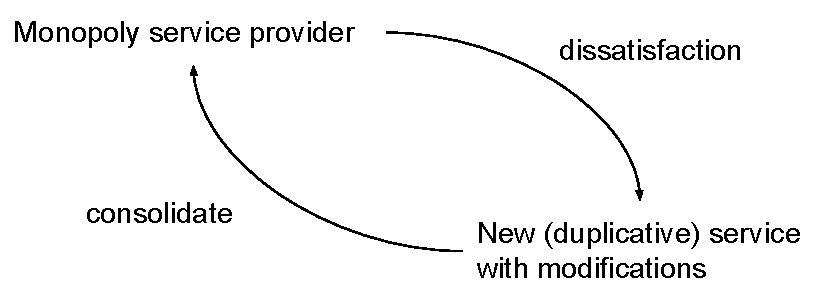
\includegraphics[width=0.8\textwidth]{images/dilemma_market_vs_monopoly.pdf}
    \caption{Dipole oscillation: solution A exists but doesn't meet my needs. Rather than tweak A, re-invent solution B which mostly overlaps with A but has independent development and support. See also Table~\ref{table:market-vs-monopoly}.}
    \label{fig:market-vs-monopoly}
\end{figure}

% https://graphthinking.blogspot.com/2021/12/hierarchical-organization-trilemma.html
Being a member of a team that operates within a hierarchy is tough. One reason is the question of who you are working for. The trilemma is whether you work for yourself, work for your supervisor, or work for your team.  Ideally you can find ways to do all three, but that is not always the case. 

Members of the team should work collaboratively, but there is a potential counter-force: accountability to the supervisor. Because each team member is accountable to their supervisor(s), that motivates the action of the individual. The team does not actually have autonomy -- they are accountable to the boss.

In the approach "team members are directed by their supervisor," the synergy of the team is neglected and the supervisor becomes a bottleneck (for decision making and for creativity and for planning).

The third approach is for a person to ignore their team and their supervisor. This might enable quicker progress, at the risk of going in an unhelpful direction or not leveraging skills of coworkers. 

\ \\

A trilemma applicable to many situations is that options are \textbf{fast, inexpensive, good; choose two}. (This is the \href{https://en.wikipedia.org/wiki/Project_management_triangle}{Project management triangle}.) \\
In other words, the options are
\begin{itemize}
    \item good and fast is expensive (i.e., requires lots of resources)
    \item good and inexpensive takes a long time (i.e., a clever solution)
    \item fast and inexpensive will be low quality
\end{itemize}

\begin{center}
\begin{figure}[ht]
    \centering
    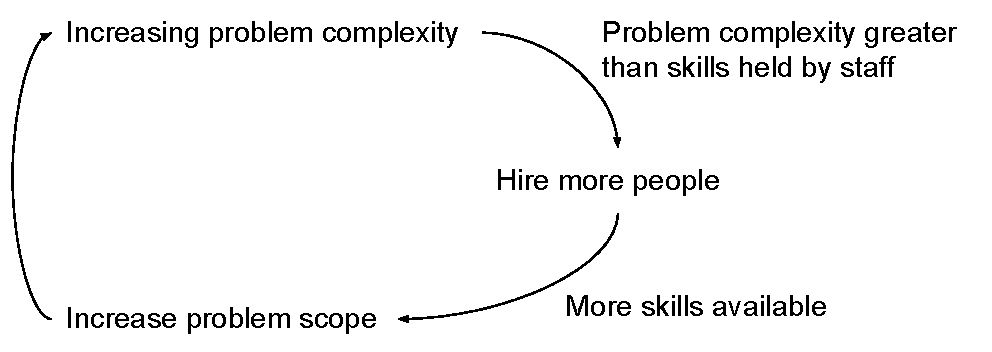
\includegraphics[width=0.8\textwidth]{images/feedback_loop_complexity_and_staffing}
    \caption{Complexity requires more staffing; having more staff means more skills are available; under-utilized staff skills make room for more scope; more scope adds to complexity.}
    \label{fig:complexity_and_staff_growth}
\end{figure}
\end{center}
